% Chapter Template

\chapter{Abast del projecte} % Main chapter title

\label{Abast} % Change X to a consecutive number; for referencing this chapter elsewhere, use \ref{ChapterX}

La idea d’aquest projecte és crear una aplicació referència per qualsevol persona disposada a emprendre un viatge. Una plataforma on trobar suport durant un viatge de qualsevol tipus.\\

L’aplicació ofereix, aprofitant d’altres sistemes ja al mercat, un conjunt de funcionalitats útils a l’hora de viatjar. Les funcionalitats són les següents:
\begin{itemize}
\item{Gestió econòmica:} Controlar qui ha pagat què durant un viatge en grup o bé
el control de les despeses del viatge de manera personal.
\begin{itemize}
\item{}Quan es crea una nova despesa s’envia un avís al deutor.
\item{}Despesa total del viatge.
\end{itemize}
\item{}Gestió de notes: Guardar notes per tal de recordar anècdotes o fets concrets
del viatge.
\begin{itemize}
\item{}Les notes tenen localització geogràfica.
\item{}Possibilitat d’etiquetar viatgers a les notes.
\end{itemize}
\item{}Gestió de cerques: Cerca de llocs d’interès de la zona on està situat l’usuari o de qualsevol altre punt.
\begin{itemize}
\item{}Cerca de restaurants.
\item{}Cerca de bars.
\item{}Cerca de llocs d’interès lúdic.
\item{}Cerca de botigues.
\item{}Cerca de llocs exteriors d’interés.
\item{}Consulta de la ruta fins al punt trobat.
\end{itemize}
Els resultats que s’obtenen de la cerca es mostren a l’usuari ordenats d’acord amb l’estil de viatjar que té l’usuari. Per fer això, abans de començar el viatge, l’aplicació proposa un formulari per tal de descriure el caràcter del viatge. Això dona l’opció al sistema de filtrar les cerques i proposar a l’usuari les opcions més adequades al seu estil.

\item{}Gestió d’emergències: Suport en cas d’emergència tenint en compte el país.
\begin{itemize}
\item{}Ruta fins a l’hospital més proper.
\item{}Trucada al telèfon d’emergències del país.
\item{}Trucada al contacte d’emergències.
\end{itemize}
En aquesta funcionalitat es vol donar la possibilitat a l’usuari de contactar amb una persona de confiança en cas d’emergència. Per aconseguir això, quan s’inicia el viatge, es presenta a l’usuari un formulari on s’han d’introduir el nom, el número de telèfon i el correu electrònic de qui serà la persona de contacte.

\item{}Previsió metereològica: Estar informat de la metereologia en tot moment.
\begin{itemize}
\item{}Predicció setmanal.
\item{}Informació metereològica del dia.
\end{itemize} 
\end{itemize}

\section{Obstacles i riscs}

Per tal d’aconseguir certes funcionalitats de l’aplicació es vol accedir a diferents serveis web per tal d’aconseguir dades concretes. Per una banda, és necessitarà connexió a internet sempre que s’hi vulgui accedir, i per l’altra, el funcionament de l’aplicació depén de la disponibilitat del servei web.\\

En el cas de les trucades d’emergència al telèfon d’emergències del país on estigui el viatger, pot ser que es trobi en un país on no hi ha dades registrades sobre els telèfons d’emergència. Un problema molt semblant pot passar a l’hora d’obtenir llocs d’interés, ja que l’usuari es pot trobar en un lloc on no hi ha cap punt ens molts quilòmetres a la rodona.\\

En ser un Treball Final de Grau té una data límit fixada. Això implica que qualsevol contratemps que faci endarrerir el projecte no es té gaire marge de maniobra per tal d’acabar-lo a temps.\\

Pel que fa a l’ús del sistema, un cop acabat i posat en marxa, s’ha de pronosticar quin tipus de situacions es podrien donar que comprometessin l’èxit del sistema. A continuació es mostra una llista de riscs que el sistema es pot trobar un cop es posi en funcionament.

\begin{itemize}
\item{}Nivell baix de bateria.
\item{}Consum de dades a l’estranger.
\item{}Caiguda del servei web.
\item{}Caiguda de la base de dades.
\item{}Canvis en la legislació.
\item{}Desconfiguració de l’aplicació.
\item{}Canvis en la resposta del servei web.
\end{itemize}

Finalment, a l’autor poden sorgir-li obstacles com: l’aparició de noves funcionalitats o canvis en les actuals que obliguen a reestructurar tot el projecte, problemes provocats per tenir poca experiència amb les tecnologies utilitzades, llenguatges de programació o una mala planificació.

\section{Metodologia}

En el desenvolupament del projecte s’utilitza la metodologia Scrum. El temps de desenvolupament està dividit en diferents sprints de dues setmanes, d’aquesta manera el treball és constant. La primera part del projecte es basa en la definició dels requisits i la definició de les històries d’usuari.\\

Per tal de garantir qualitat en la feina feta, cada setmana en acabar l’sprint, es fa una revisió de les tasques acabades i una valoració del treball fet assegurant que tot estigui correcte. Per acabar es planifica el següent sprint. Un punt molt important que fa que utilitzar aquesta metodologia sigui bo pel projecte és que es tracta de que a cada iteració s’implementin funcionalitats que puguin ser entregades al client. Per
tant, des del primer sprint tindrem una aplicació que funciona i hi anirem afegint funcionalitats. D’aquesta manera podem comprovar si el que estem desenvolupant és el que realment es necessita i fer els canvis necessaris si no estem anant per bon camí. A més, també podem detectar problemes en les parts ja implementades i així solucionar-los en les pròximes iteracions.\\

Per tal de seguir aquesta metodologia s’utilitza l’eina Trello. Trello és un software d’administració de projectes amb interfície web, iOS i Android. En aquest projecte s’utilitza aquesta aplicació per tal d’organitzar els sprints setmanals de manera visual i intuïtiva.\\

Per tal d’assegurar-nos la persistència del codi i tenir-lo guardat al núvol s’utilitza Git amb la plataforma GitHub. GitHub és un servei de hosting de repositoris Git, el qual ofereix tota la funcionalitat de Git de control de revisió distribuït i administració de codi font, i a més, també afegeix les seves característiques pròpies.


\section{Eines de seguiment}

Per tal de portar un control de la feina feta s’utilitzen diferents eines de seguiment. En la part d’implementació, durant les iteracions, s’utilitza la eina Toggl. Toggl és un software disponible a la xarxa que permet portar el control del temps que dediques a una tasca en concret. Per tant, a cada historia d’usuari que es comença se li assigna una nova tasca i es fica el cronòmetre en marxa. A la figura 2.1 es pot veure
un exemple d’utilització de l’eina.\\

Una altra eina de seguiment és la preparació de les reunions amb la tutora del projecte, normalment, una reunió al final de cada iteració. A l’inici de cada sprint, com a planificació d’aquest, es redacta un informe on hi apareix l’esquema de casos dús on es pot diferenciar entre els que han sigut implementats, els que es preten implementar en l’sprint i els que queden pendents; un anàlisi de les tecnologies que s’han d’utilitzar durant la iteració (APIs, serveis externs, etc) i l’especificació dels
casos d’ús que es volen implementar en la iteració.\\

Quan s’acaba una iteració, a mode de resum, també es redacta un document
valorant la feina que s’ha fet i remarcant qualsevol aspecte important per la implementació del projecte.

\begin{figure}[!h]
\centering
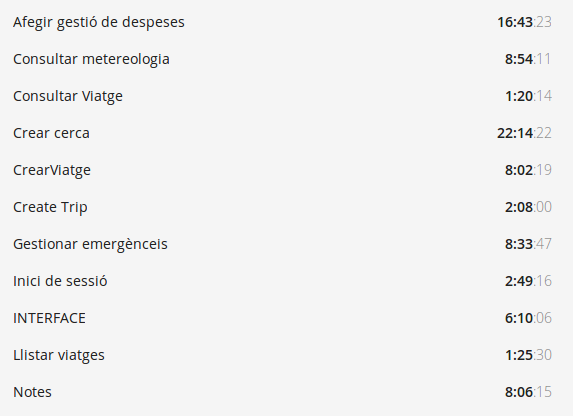
\includegraphics[scale=0.65]{Figures/toggl.jpg}
\caption{Resum de tasques a Toggl.}
\end{figure}

\section{Adequació a Enginyeria del Software}

Aquest projecte és un treball de final de grau de modalitat A, l’alumne proposa una idea i la desenvolupa. En aquest cas la idea que pretén desenvolupar aquest projecte és una aplicació mòbil de suport al viatger. En ser una aplicació mòbil el projecte necessita un bon disseny a nivell de software, cosa que requereix comptar amb un dissenyador amb coneixements prou avançats d’enginyeria del software. Aconseguir un bon disseny permetrà obtenir una aplicació sòlida, neta i molt fàcil de
mantenir.\\

Un altre punt important d’aquest projecte és que es caracteritza per utilitzar aplicacions ja existents en el mercat. Això significa que és necessari dissenyar l’aplicació de tal manera que permeti utilitzar serveis que estan disponibles al núvol.\\

A més, en el món dels serveis web hi ha avanços molt sovint i surten noves
aplicacions cada cert període de temps. És per això que aquesta aplicació vol estar preparada per tal d’assumir canvis pagant el preu més baix possible. Per tant, aquesta aplicació pretén ser dissenyada de manera que sigui molt senzill adjuntar noves funcionalitats o eliminar alguna de les existents, és a dir, pretén potenciar l’escalabilitat.

\subsection{Competències tècniques del projecte}
\begin{itemize}
\item{}CES1.1: Desenvolupar, mantenir i avaluar sistemes i serveis software complexos i/o crítics. [En profunditat]\\
És l’essència del projecte ja que es tracta de desenvolupar i mantenir un servei software d’una certa complexitat. Aquesta competència s’assoleix amb el desenvolupament complet del projecte.
\item{}CES1.2: Donar solució a problemes d’integració en funció de les estratègies, dels estàndards i de les tecnologies disponibles. [Una mica]\\
L’aplicació necessita la participació d’aplicacions externes per tal  d’aconseguir certes funcionalitats, per tant, és necessàri la integració de les dades que arriben des dels serveis exteriors.
\item{}CES1.3: Identificar, avaluar i gestionar els riscos potencials associats a la construcció de software que es poguessin presentar. [Bastant]\\
Aquest objectiu s’assoleix durant l’estudi de viabilitat del projecte ja que s’ha de preveure quins seran els possibles riscos a l’hora del desenvolupament.
\item{}CES1.5: Especificar, dissenyar, implementar i avaluar bases de dades. [Una mica]\\
Per dur a terme aquest projecte serà necessari el desenvolupament d’una ba-
se de dades, per tant, amb el disseny i desenvolupament d’aquesta s’assolirà aquesta competència.
\item{}CES1.6: Administrar bases de dades (CIS4.3) [Una mica]\\
Un cop l’aplicació estigui posada en marxa s’haurà d’administrar la base de
dades, per aquest motiu la competència no incideix en profunditat. Aquesta
competència s’assolirà un cop acabat el projecte.

\item{}CES1.7: Controlar la qualitat i dissenyar proves en la producció de software. [En profunditat]\\
En utiltizar una metodologia Agile es dona molta importància al control de
qualitat i a les proves durant el desenvolupament, aquesta competència es posarà a prova en profunditat durant el desenvolupament del producte.
\item{}CES1.9: Demostrar comprensió en la gestió i govern dels sistemes software. [En profunditat]\\
Desenvolupar una aplicació com aquesta requereix d’una bona gestió del sistema software, per aquest motiu es treballa aquesta competència en profunditat i s’assoleix havent acabat el projecte amb èxit.
\item{}CES2.1: Definir i gestionar els requisits d’un sistema software. [En profunditat]\\
Durant l’especificació de requisits es quan es treballa i s’assoleix aquesta competència, és una part bàsica del projecte i per aquest motiu es treballa en profunditat.
\item{}CES2.2: Dissenyar solucions apropiades en un o més dominis d’aplicació, utilitzant mètodes d’enginyeria del software que integrin aspectes ètics, socials, legals i econòmics. [En profunditat]\\
En el desenvolupament del projecte és necessari dissenyar solucions apropiades utilitzant mètodes d’enginyeria del software, s’assolirà aquesta competència en profunditat havent acabat el projecte amb èxit.
\end{itemize}

\subsection{Coneixements Aplicats}
Durant la meva estada a la FIB he cursat vàries assignatures amb continguts molt interessants a l’hora de desenvolupar aquest projecte. En especial, les que més s’apliquen en aquest projecte a nivell tècnic són:
\begin{itemize}
\item{}\textbf{AS:} Tots els continguts tècnics d’arquitectura de software.
\item{}\textbf{GPS:} En aquesta assignatura es va treballar la gestió de projectes, en aquest cas, la part d’Agile és la més important.
\item{}\textbf{PES:} Durant el desenvolupament del projecte d’especialitat es va fabricar una aplicació Android com la que es desenvolupa en aquest projecte. A més es van utilitzar mètodes de seguiment i metodologia que s’aplica a aquest projecte.
\item{}\textbf{ASW:} Aquesta aplicació necessita utilitzar serveis web, cosa que es va exposar en l’assignatura ASW.
\item{}\textbf{ER:} Durant l’especificació de requisists s’ha utilitzant en tot moment els coneixements adquirits cursant aquesta assignatura.
\item{}\textbf{BD:} Per tal de dissenyar la base de dades s’ha posat en pràctica part dels coneixements adquirits a l’assignatura.
\item{}\textbf{CBDE:} Per tal de dissenyar la base de dades s’ha posat en pràctica els coneixements i l’esperit crític adquirit a l’assignatura sobre les bases de dades no relacionals.

\end{itemize}
